\chapter{Implémentation du système}
\chaptermark{Système}
\minitoc
\newpage

\section{Introduction}

Comme nous l'avons expliqué dans les parties précédentes de notre mémoire, la problématique de notre sujet est de faire de la prédiction  de matériels informatiques plus des ordinateurs afin de savoir éventuellement ceux qui sont susceptibles de tomber en panne. Il s'agit de prédiction de données quantitatives et qualitatives.

\section{Expérimentations et résultats}
Pour mettre en place notre solution, nous aurons plusieurs étapes notamment les étapes de nettoyage, de préparation  de données, et de machine learning. Après étude de l'état de l'art, nous avons donc décidé d'appliquer comme algorithmes, les Arbres de Décision, les Random Forest et la Regression Logistique.  Pour rappel, pour obtenir notre jeu de données final nous avons effectué des étapes de consolidation et d'aggrégation de plusieurs jeux de données d'historisation sur des matériels informatiques. Ci-dessous, les étapes de notre travail.

\subsection{Expérimentations}

\begin{itemize}[label=\textbullet, font=\LARGE \color{black}]
\item Chargement du jeu de données brutes
\begin{figure}[h]
\begin{center}
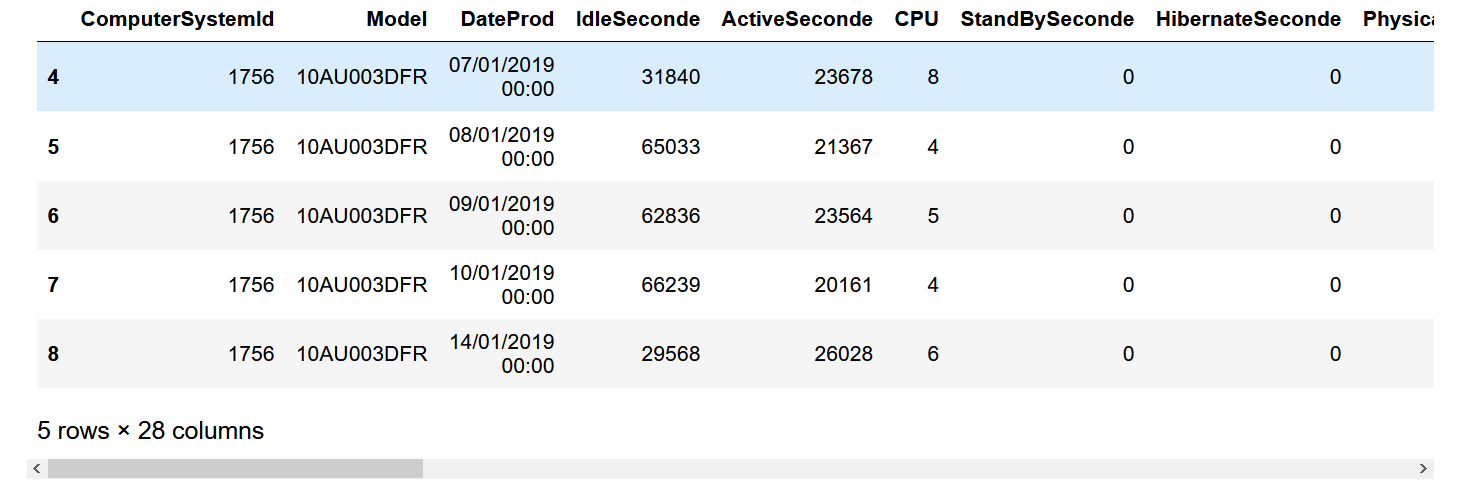
\includegraphics[scale=0.50]{Donnes_brutes.png}
\caption[Jeu de données sur des caractéritiques d'ordinateurs loués]{Jeu de données sur des caractéritiques d'ordinateurs loués}
\label{monlabel}
\end{center}
\end{figure}
\newline
La Figure nous montre quelques colonnes de notre jeu de données après y avoir fait les étapes de consolidation de table. Il s'agit d'un jeu de 28 colonnes avec une colonne de type date (DateProd) et une colonne de type chaine de caractères (Model). C'est cette dernière colonne que nous  allons prédire.

\newpage
\item Répartition des modèles d'ordinateur.
\newline
\begin{figure}[h]
\begin{center}
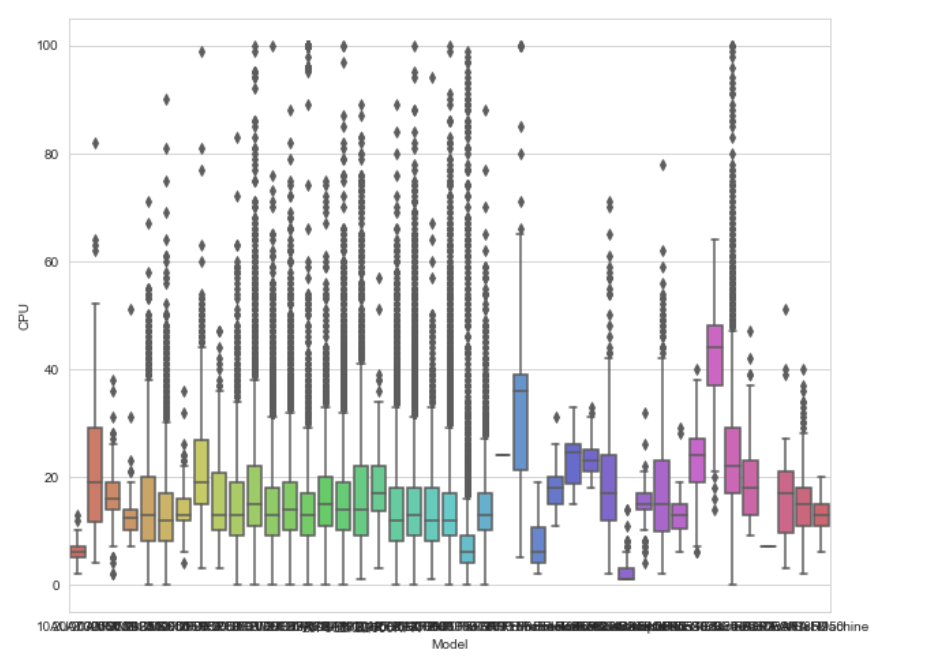
\includegraphics[scale=0.90]{Box_plot_repartition.png}
\caption[Boite à moustache]{Boite à moustache}
\label{monlabel}
\end{center}
\end{figure}
\newline
Cette figure montre une répartition des modèles d'ordinateurs en fonction du processeur

\newpage
\item Histogramme sur les nombres d'ordinateurs par modèle
\newline
\begin{figure}[h]
\begin{center}
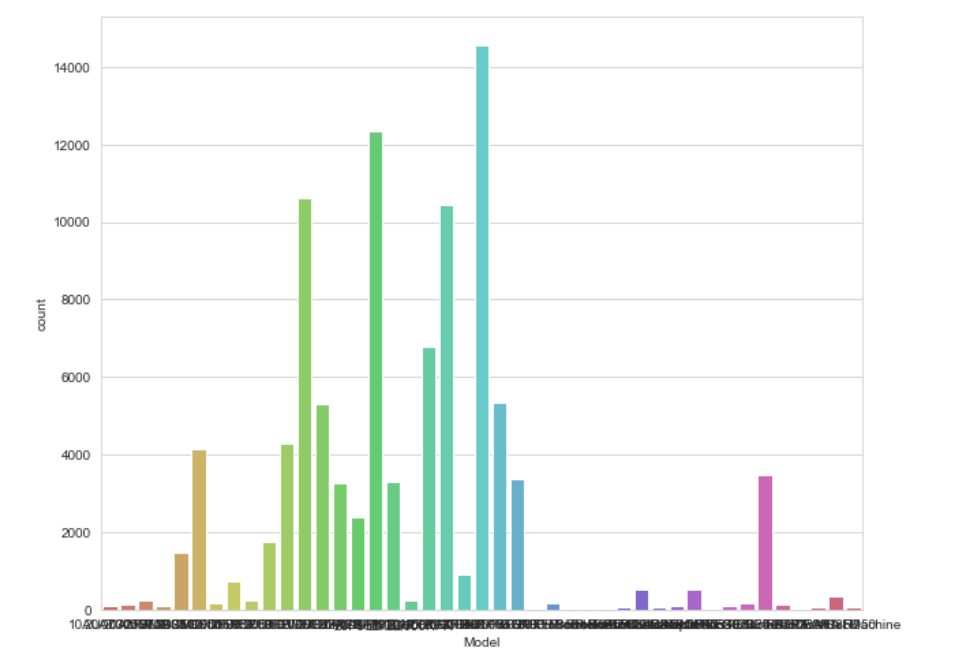
\includegraphics[scale=0.80]{Dataviz_model_count.png}
\caption[Histogramme sur les nombres d'ordinateur spar modèle]{Histogramme sur les nombres d'ordinateurs par modèle}
\label{monlabel}
\end{center}
\end{figure}

\newpage
\item Description du jeu de données préparées et nettoyées pour l'apprentissage
\newline
Les caractéristiques du jeu de données nous montre types des colonnes. Pour ce jeu de données, nous avons eu à supprimer les lignes de données manquantes, à faire des conversion des formats, par exemple des type float en interger comme c'est le cas de plusieurs colonnes. Nous avons également enrichi nos données avec deux colonnes supplémentaires, une colonne \textbf{Size\_Model} qui transforme et affecte des numéros de classe à chaque valeur de la colonne Model, une seconde colonne NumberDays qui constitue le nombre de jours d'inactivité de l'ordinateur. Cette dernière colonne importante nous permettra donc avec les autres colonnes caractéristiques de l'ordinateur de prédire les modèles d'ordinateur qui vont tomber en panne.
\begin{figure}[h]
\begin{center}
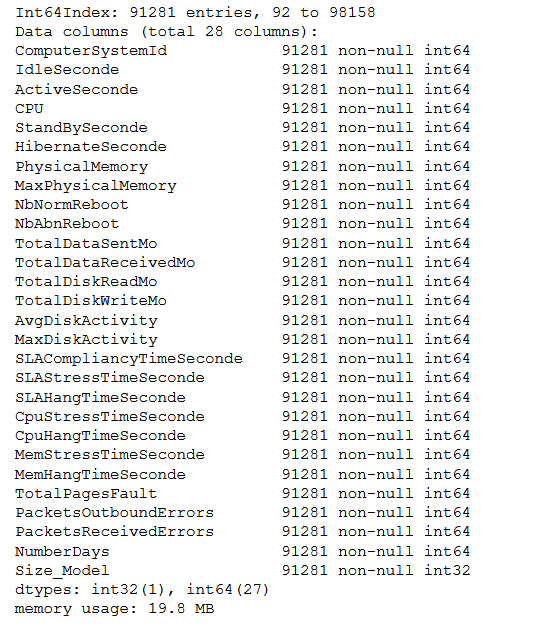
\includegraphics[scale=0.90]{Description_Donnees_apprentissage.png}
\caption[Description du jeu de données préparées]{Description du jeu de données préparées}
\label{monlabel}
\end{center}
\end{figure}


\newpage
\item Matrice de corrélation entre les variables
\newline
La matrice ci-dessus présente les relations de lien encore appelées corrélations entre les différentes variables  de notre jeu de données.
\begin{figure}[h]
\begin{center}
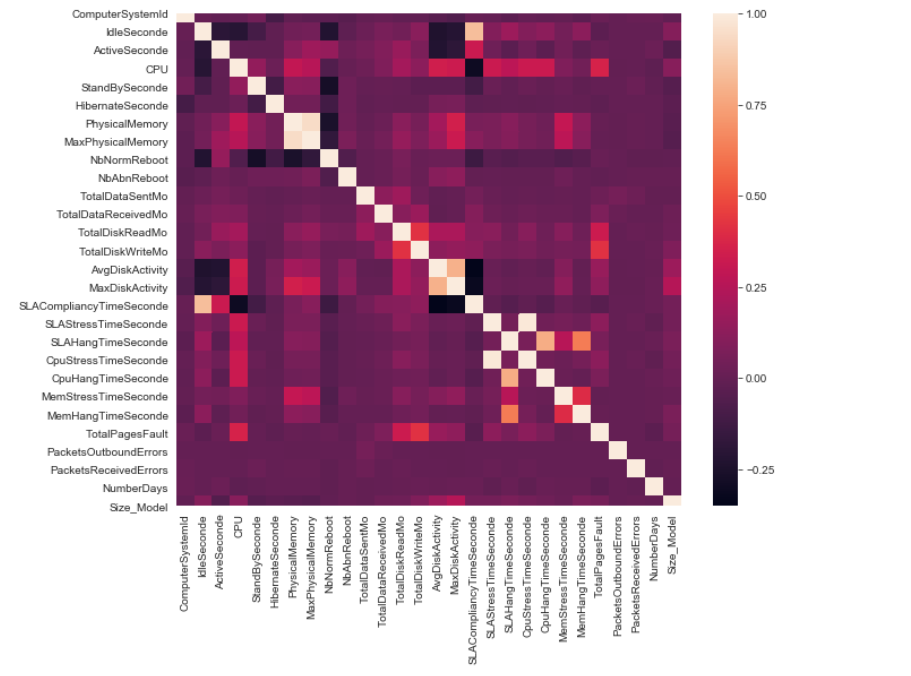
\includegraphics[scale=0.90]{Matrice_correlation.png}
\caption[Matrice de corrélation entre les variables]{Matrice de corrélation entre les variables}
\label{monlabel}
\end{center}
\end{figure}
\newline
La matrice de corrélation nous a permis de vérifier si nécessaire que nous a permis de mieux analyser nos données afin de voir si eventuellement il y a des varibales à forte corrélation avec d'autres variables. Si c'est le cas ces variables ne seront pas gardées pour l'apprentissage car elle ne permettront pas de donner de bons résultats.

\newpage
\item Comparaison des algorithmes
\newline
La figure ci-dessus compare les scores d'apprentissage des trois algorithmes que nous avons appliqué sur notre jeu de données notamment le Random Forest, les Arbres de Décision et La Regression Logistique.
\begin{figure}[h]
\begin{center}
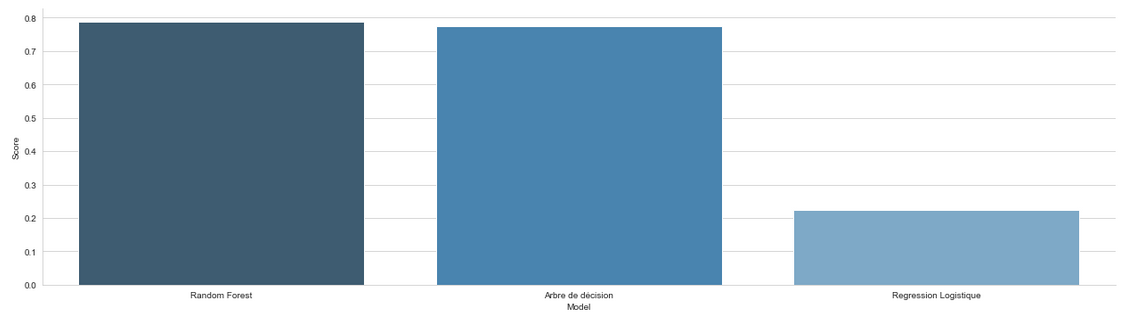
\includegraphics[scale=0.70]{Resultats_scoring.png}
\caption[Comparaison des algorithmes]{Comparaison des algorithmes}
\label{monlabel}
\end{center}
\end{figure}
\end{itemize}
Nous pouvons conclure que le Random Forest donne des résultats meilleurs par rapport aux deux autres algorithmes que sont les Arbres de Décision et la Regression Logistique.


\section{Conclusion}
Au cours de ces expérimentations, nous avons donc eu à manipuler et traiter nos données de différentes manières. Toutefois les étapes de pré-traitement nous ons permis notamment d'enrichir nos données, de les nettoyer afin d'obtenir des résultats relativement bonnes pour la phase d'apprentissage.